\documentclass{beamer}
\usepackage{pgfpages}
%\setbeameroption{show notes on second screen=left} %enable for notes
\usepackage{graphicx}
\usepackage{xcolor}
\usepackage{listings}
\usepackage{hyperref}
\lstset{language=python,frame=single}
\usepackage{verbatim}
\usepackage{apacite}
\usepackage{subcaption}
\usepackage{amsmath}
\usepackage{relsize}
\usepackage{appendixnumberbeamer}
\usepackage{xparse}
\usepackage{multimedia}
\usepackage{tikz}
\usetikzlibrary{matrix,backgrounds}
\usetikzlibrary{positioning}
\pgfdeclarelayer{myback}
\pgfsetlayers{myback,background,main}

\tikzset{
  invisible/.style={opacity=0},
  visible on/.style={alt={#1{}{invisible}}},
  alt/.code args={<#1>#2#3}{%
    \alt<#1>{\pgfkeysalso{#2}}{\pgfkeysalso{#3}} % \pgfkeysalso doesn't change the path
  },
}
\tikzset{mycolor/.style = {line width=1bp,color=#1}}%
\tikzset{myfillcolor/.style = {draw,fill=#1}}%
\tikzset{ 
    table/.style={
        matrix of nodes,
        row sep=-\pgflinewidth,
        column sep=-\pgflinewidth,
        nodes={
            rectangle,
            draw=black,
            align=center
        },
        minimum height=1.5em,
        text depth=0.5ex,
        text height=2ex,
        nodes in empty cells,
%%
        every even row/.style={
            nodes={fill=gray!20}
        },
    }
}
\def\myletdropspace{0.05cm}

\NewDocumentCommand{\highlight}{O{blue!40} m m}{%
\draw[mycolor=#1,rounded corners] (#2.north west)rectangle (#3.south east);
}

\NewDocumentCommand{\fhighlight}{O{blue!40} m m}{%
\draw[myfillcolor=#1,rounded corners] (#2.north west)rectangle (#3.south east);
}

\usetheme[numbering=fraction]{metropolis}
%%\AtBeginSection[]
%%{
%%  \begin{frame}
%%    \frametitle{Table of Contents}
%%    \tableofcontents[currentsection]
%%  \end{frame}
%%}

%%\let\olditem\item
%%\renewcommand{\item}{\vspace{0.5\baselineskip}\olditem}
\begin{document}

\title{Finding the words}
\subtitle{One-shot and few-shot learning of word embeddings}
\author{Andrew Lampinen}
\date{CSLI, 9/12/2017}
\frame{\titlepage}

\begin{frame}{One-shot word learning}
\begin{columns}
\begin{column}{0.5\textwidth}
\textit{’Twas brillig, and the slithy toves}\\
\textit{Did gyre and gimble in the wabe:}\\ 
\textit{All mimsy were the borogoves,}\\
\textit{And the mome raths outgrabe.}\\[10pt]

\textit{“Beware the Jabberwock, my son! }\\
\textit{The jaws that bite, the claws that catch!}\\
\textit{Beware the Jubjub bird, and shun}\\ 
\textit{The frumious Bandersnatch!” }\\[10pt]

\textit{He took his vorpal sword in hand}\\
\textit{[...]}
\end{column}
\begin{column}{0.5\textwidth}
\centering
\includegraphics[height=0.8\textheight]{figures/Jabberwocky.jpg}
\end{column}
\end{columns}
\end{frame}

\begin{frame}{One-shot word learning}
\centering
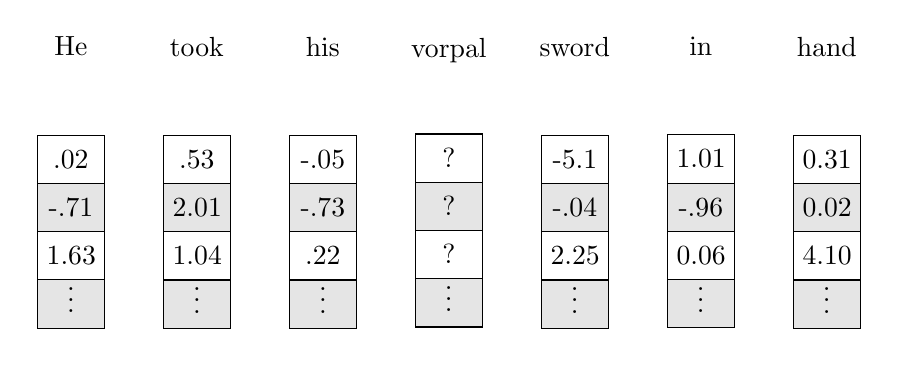
\begin{tikzpicture}
\node (w1) [visible on=<1->] {He};
\node (w2) [right=1.6cm of w1.center, anchor=center, visible on=<2->] {took};
\node (w3) [right=1.6cm of w2.center, anchor=center, visible on=<3->] {his};
\node (w4) [below right=\myletdropspace and 1.6cm of w3.center, anchor=center, visible on=<4->] {vorpal};
\node (w5) [above right=\myletdropspace and 1.6cm of w4.center, anchor=center, visible on=<5->] {sword};
\node (w6) [right=1.6cm of w5.center, anchor=center, visible on=<6->] {in};
\node (w7) [right=1.6cm of w6.center, anchor=center, visible on=<7->] {hand};

\matrix (v1) [table, text width=1.75em, below=0.75cm of w1, visible on=<1->] {
.02 \\
-.71 \\
1.63 \\
\vdots \\
};
\matrix (v2) [table, text width=1.75em, below=0.75cm of w2, visible on=<2->] {
.53 \\
2.01 \\
1.04 \\
\vdots \\
};
\matrix (v3) [table, text width=1.75em, below=0.75cm of w3, visible on=<3->] {
-.05 \\
-.73 \\
.22 \\
\vdots \\
};
\matrix (v4) [table, text width=1.75em, below=0.65cm of w4, visible on=<4->] {
? \\
? \\
? \\
\vdots \\
};
\matrix (v5) [table, text width=1.75em, below=0.75cm of w5, visible on=<5->] {
-5.1 \\
-.04 \\
2.25 \\
\vdots \\
};
\matrix (v6) [table, text width=1.75em, below=0.75cm of w6, visible on=<6->] {
1.01 \\
-.96 \\
0.06 \\
\vdots \\
};
\matrix (v7) [table, text width=1.75em, below=0.75cm of w7, visible on=<7->] {
0.31 \\
0.02 \\
4.10 \\
\vdots \\
};

\end{tikzpicture}
\end{frame}
\begin{frame}{Introduction}
One-shot learning of word embeddings? 
\begin{itemize}
    \item<1-> Word-embedding based systems are achieving quite good performance on some tasks. 
    \item<2-> But humans can learn fast.
    \item<3-> Can CLS resolve this?
\end{itemize}
\end{frame}


\begin{frame}{Background}
Surprisingly little work on one-shot learning of embeddings:
\begin{itemize}
    \item<1-> \cite{Lazaridou2017} -- One-shot word learning in a multi-modal setting. 
    \item<2-> Work from Erk \& colleagues \cite{Wang2017}, which we'll hear about later -- Not embeddings, but has some relation.
\end{itemize}
\end{frame}

\section{Approach}
\begin{frame}{task}

\end{frame}

\begin{frame}{Model}

\end{frame}

\begin{frame}{Conclusions}
\begin{itemize}
    \item<1-> 
\end{itemize}
\end{frame}

\begin{frame}{Future Directions}
\begin{itemize}
    \item<4-> Faster integration of schema-consistent knowedge?
\end{itemize}
\end{frame}

\begin{frame}{Acknowledgements}
Thanks to:
\begin{itemize}
    \item Jay McClelland and the rest of the lab.
    \item The NSF, for funding.
    \item You, for listening. 
\end{itemize}
\end{frame}

\begin{frame}[allowframebreaks]
\bibliographystyle{apacite}
\bibliography{one_shot_words}
\end{frame}



\end{document}
